\documentclass{article}

\usepackage{graphicx}
\usepackage[left=2cm, right=2cm, top=2cm]{geometry}

\begin{document}

% The following part of this document will be placed in the Methods section

The next test determines how well the three solvers perform for varying
coordinate systems, for constant parameters $q$ and $s$. This test is
done for the binary lens. Even though the solvers perform equally well
in the planet frame, it is worth checking how well they perform in the
other frames, as well. This will give us an idea of which solvers perform
better in general; and thus, suggest which solver ought to be used in
general microlensing computations. Again, the simulation plots the number
of images and the magnification for a plot of points in the source plane.
\textbf{Figure 1} shows the plot of the number of images, and
\textbf{Figure 2} shows the plot of the magnification.

\begin{figure}
	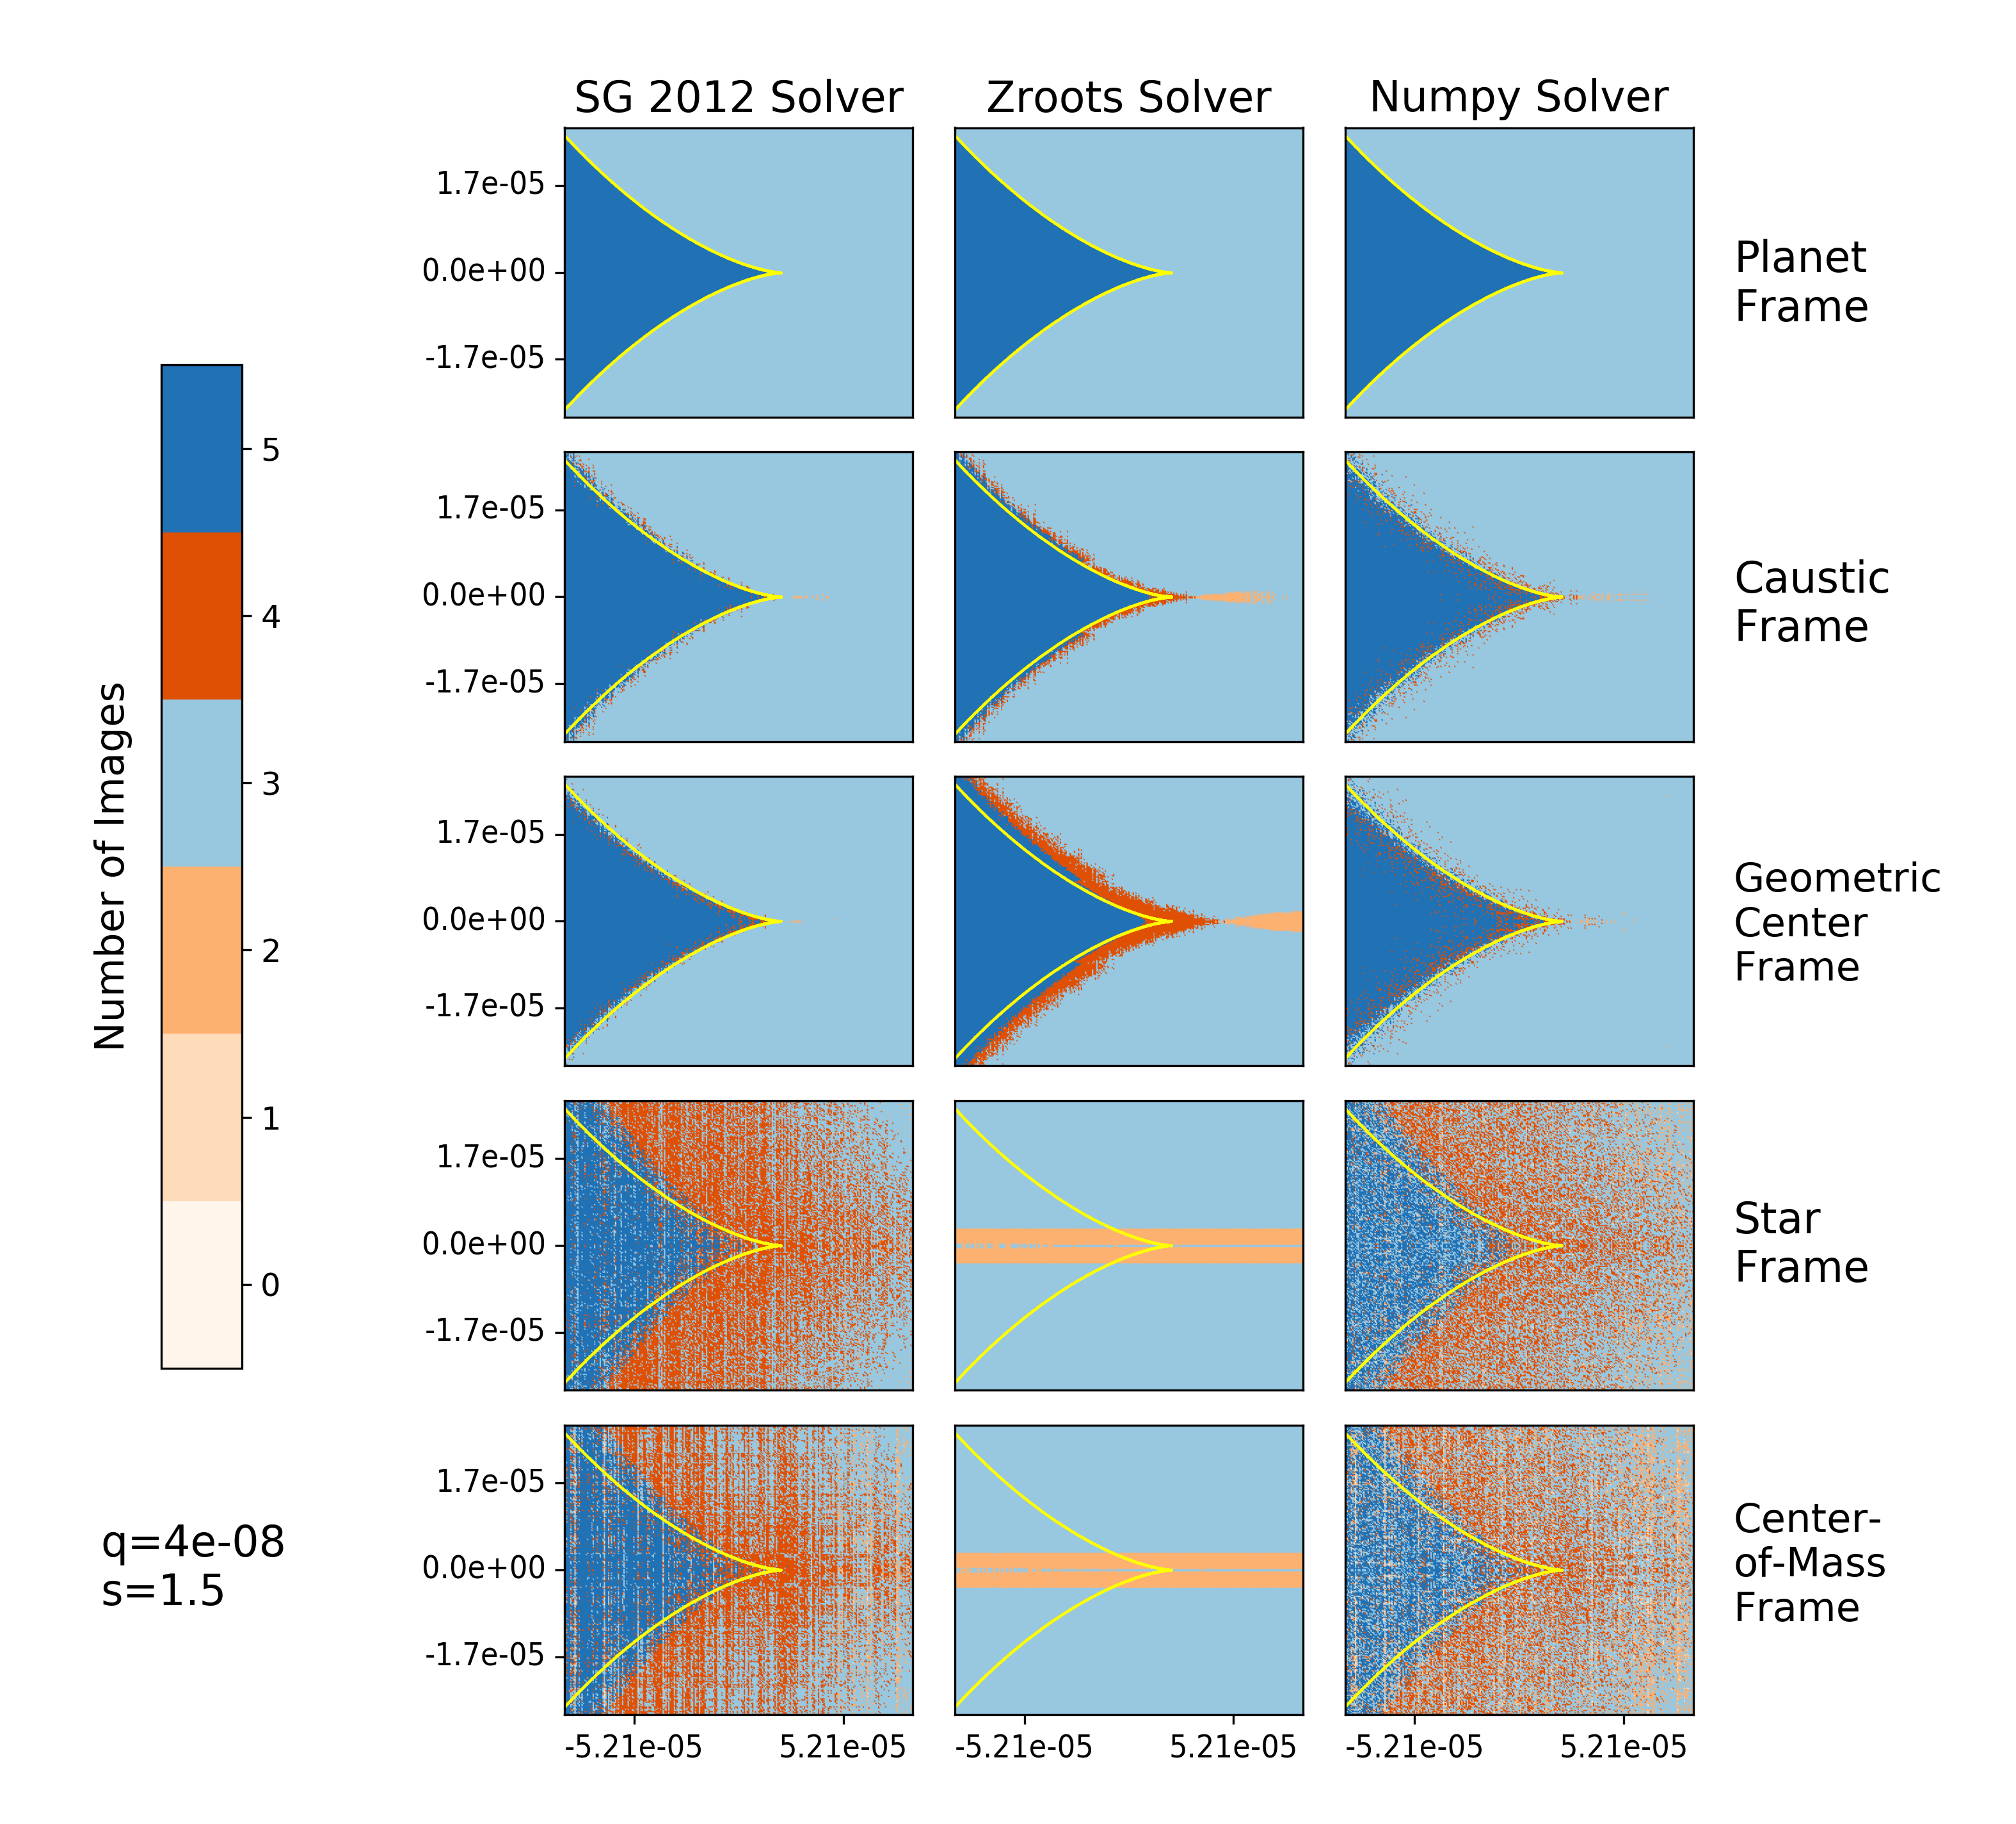
\includegraphics[width=0.9\textwidth]{../Tables/images_solver_0.png}
	\caption{The number of images versus the position for each root solver
	for a given separation and mass ratio. The rows coorespond to different
	coordinate frames. All of the plots, except for those in planet frame,
	show errors since the mass ratio, $q$ is near its lower limit for most
	frames. The planet frame plots, therefore, can be our comparison plots
	to show what we would expect for the given parameters $s$ and $q$. In
	the rest of the frames, the Skowron and Gould root solver generally
	produces the least noise and number of errors. The plots fail completely
	for the center-of-mass and star frames.}
\end{figure}

\begin{figure}
	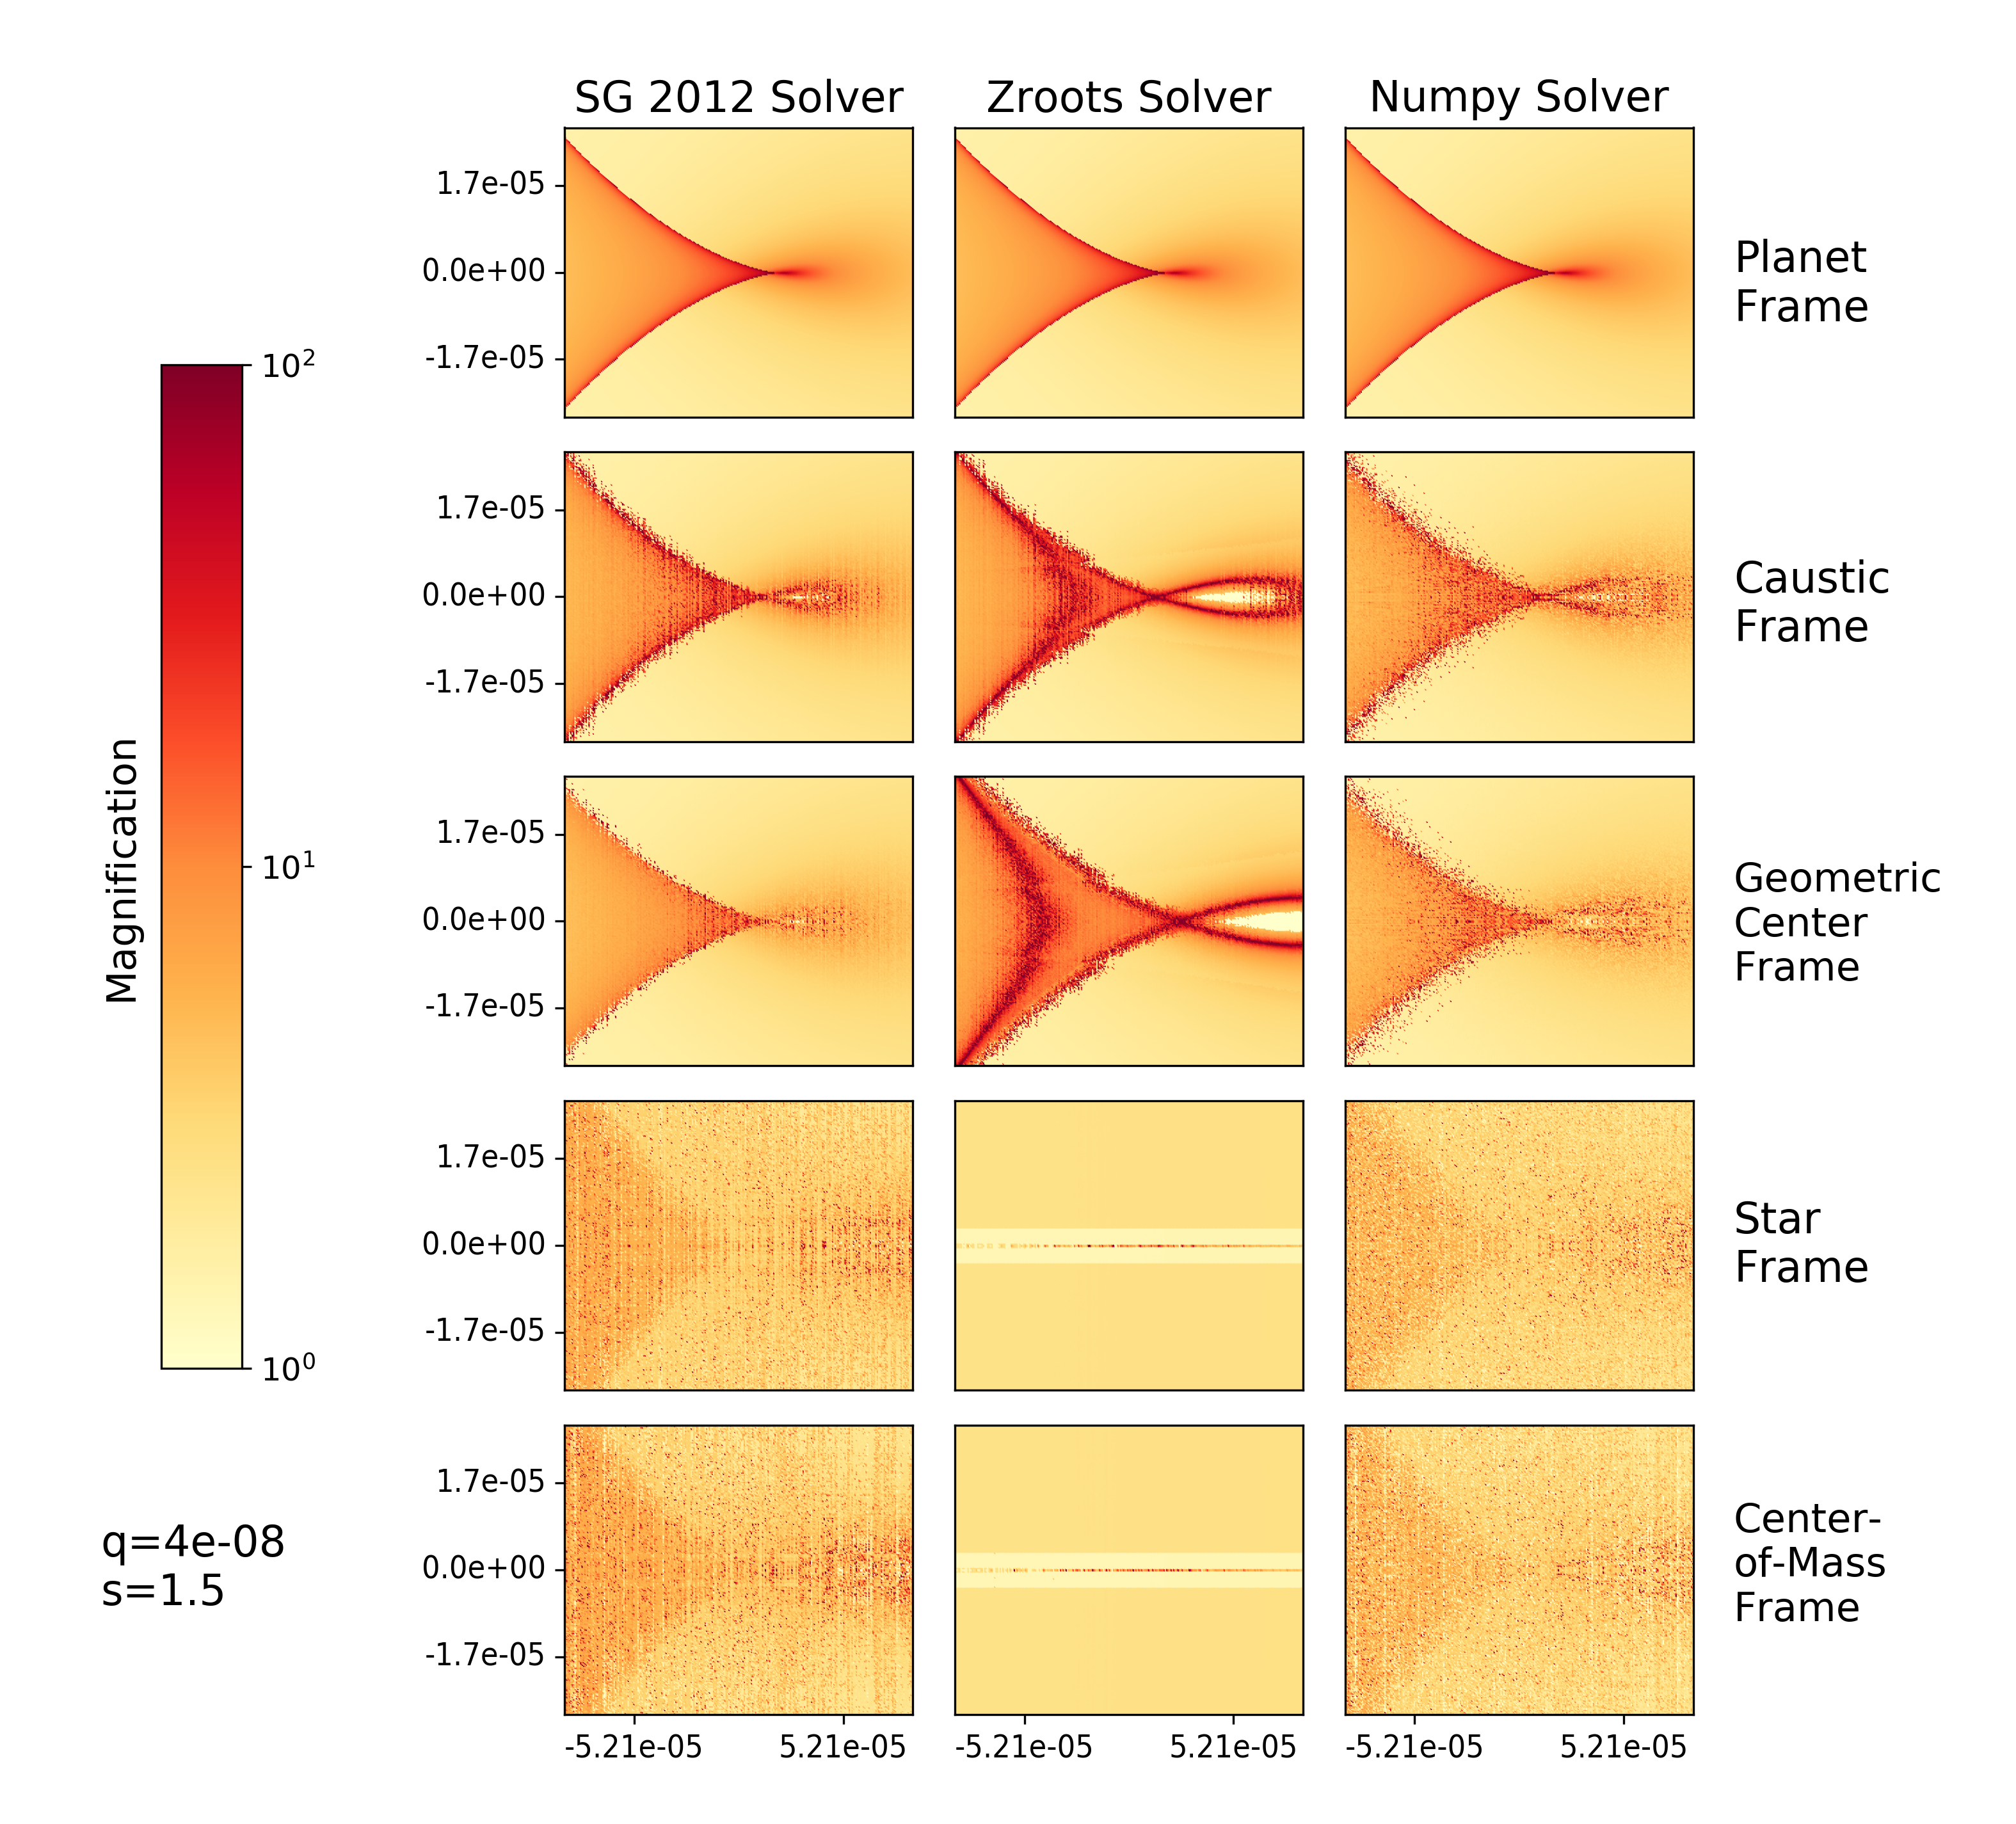
\includegraphics[width=0.9\textwidth]{../Tables/magn_solver_0.png}
	\caption{Same as \textbf{Figure 1}, except with magnification.}
\end{figure}

% The following part of this document will be placed in the Results/Analysis
% section

This simulation suggests that the Skowron and Gould 2012 root finder will
generally provide the most reliable (i.e. least error-prone) calculations. 

\end{document}
